\chapter{Figuras Complementares da Literatura Empírica} \label{anexo:currie}

Este anexo reproduz figuras de \textcite{currie2020} utilizadas apenas como contextualização da guinada empírica da economia e da difusão de métodos quase-experimentais. Elas foram deslocadas para o anexo para preservar, no corpo do texto, uma revisão de literatura mais direta e concentrada no problema de identificação deste trabalho.

\begin{figure}[htbp]
    \centering
    \caption{Artigos de Microeconomia Aplicada nas revistas \textit{Top-Five}}
    \label{fig:currie1}
    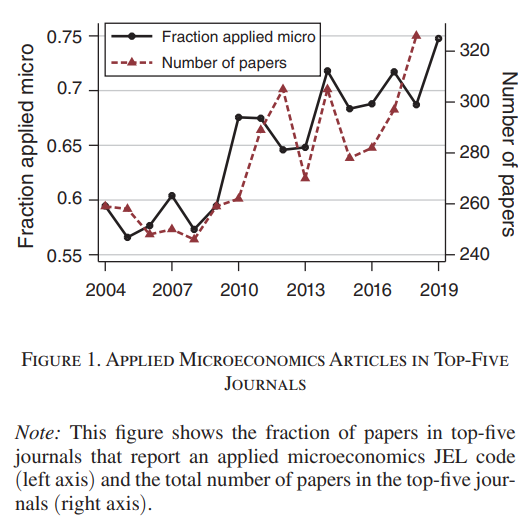
\includegraphics[width=0.7\textwidth]{tabelas/imagens/figura1currie.png}
    \\ \vspace{0.1cm}
    \footnotesize{\textbf{Fonte:} \textcite{currie2020}.}
\end{figure}

\begin{figure}[htbp]
    \centering
    \caption{Evolução do uso de métodos quase-experimentais}
    \label{fig:currie4}
    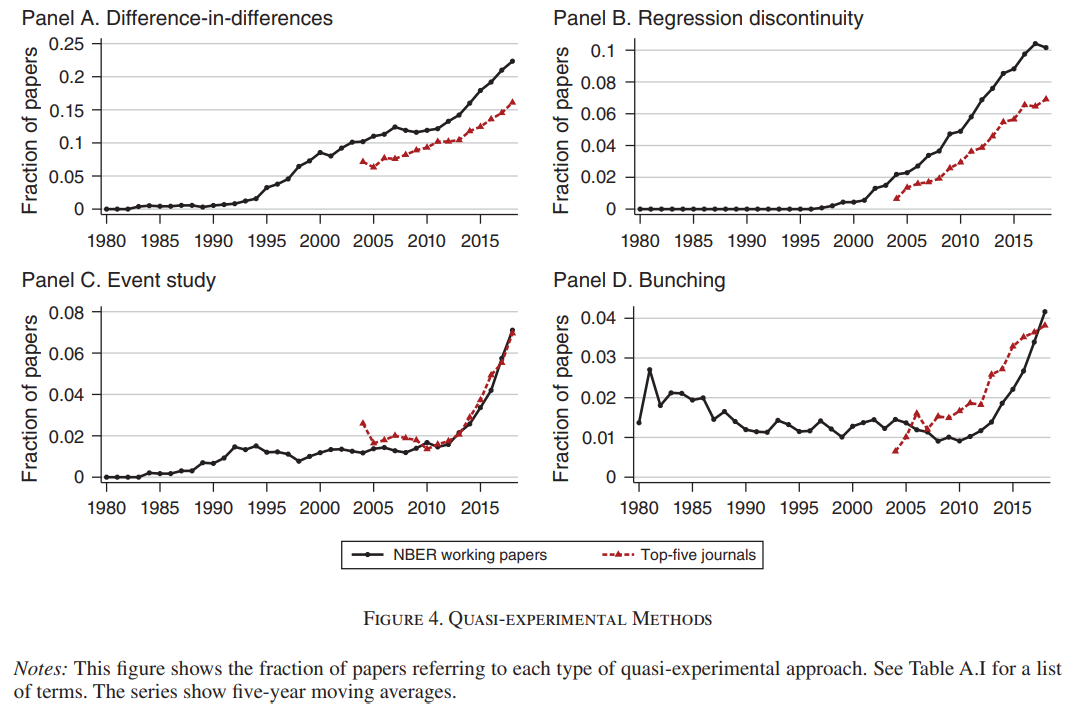
\includegraphics[width=0.9\textwidth]{tabelas/imagens/figura4currie.png}
    \\ \vspace{0.1cm}
    \footnotesize{\textbf{Fonte:} \textcite{currie2020}.}
\end{figure}

\begin{figure}[htbp]
    \centering
    \caption{Evolução do uso de termos sobre precisão de estimativas}
    \label{fig:currie5}
    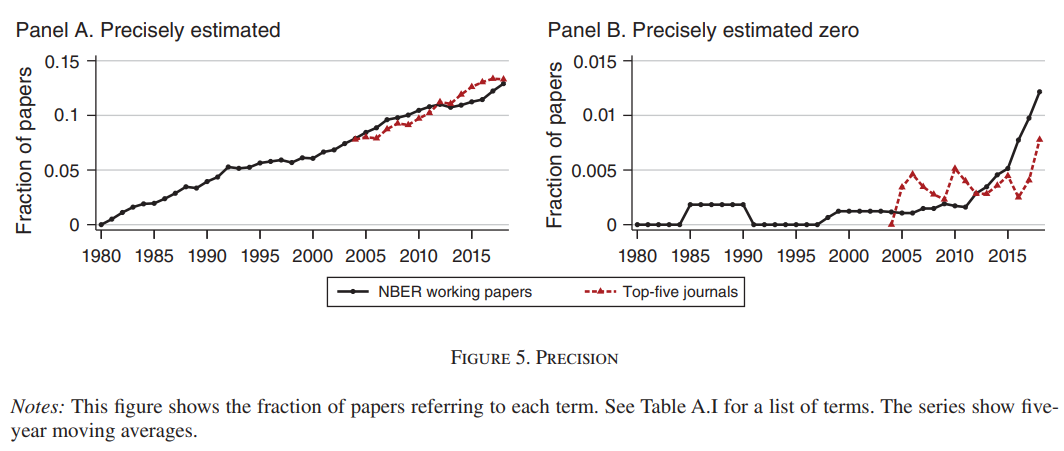
\includegraphics[width=0.9\textwidth]{tabelas/imagens/figura5currie.png}
    \\ \vspace{0.1cm}
    \footnotesize{\textbf{Fonte:} \textcite{currie2020}.}
\end{figure}
